\begin{frame}[t]%
\smallskip

\begin{exercise}{Programmentwicklung}
\begin{body}
\begin{parts}
\item Wozu dient der Java-Compiler, wozu der Java-Interpreter?
\item Erläutern Sie die Aussage \glqq Java ist plattformunabhängig\grqq.
\end{parts}

\end{body}

\begin{solution}
\begin{parts}
\item Der Java-Compiler überprüft einen Java-Quelltext auf syntaktische Korrektheit und meldet ggf. Syntaxfehler. Ist der Quelltext korrekt, so übersetzt der Java-Compiler diesen in den sogenannten Java-Bytecode. Der Java-Interpreter liest diesen Bytecode und führt ihn aus.

\item
Die Programmiersprache Java ist in zweierlei Hinsicht plattformunabhängig: auf Quelltextebene und auf Bytecode-Ebene. Ersteres bedeutet, dass ein Java-Quelltext auf jedem Rechner, unabhängig von dessen Prozessorarchitektur (IBM, Mac, etc.) und dessen Betriebssystem (MS Windows, Linux, Mac OS, etc.), in gleicher Weise übersetzt wird, ohne dass entsprechende Anpassungen vorgenommen werden müssen. Plattformunabhängigkeit auf Bytecode-Ebene bedeutet, dass der Java-Bytecode auf jedem Rechner, unabhängig von dessen Prozessorarchitektur und Betriebssystem, in gleicher Weise ausgeführt wird. Einschränkend muss gesagt werden, dass diese Aussagen nur dann richtig sind, wenn auf den verschiedenen Rechnern dieselbe Version des Java-Compilers und des Java-Interpreters installiert sind.
\end{parts}
\end{solution}
\end{exercise}

\end{frame}

\begin{frame}[t]%
  \frametitle{Unterschiede zwischen Java und C++}%
\centering
\medskip

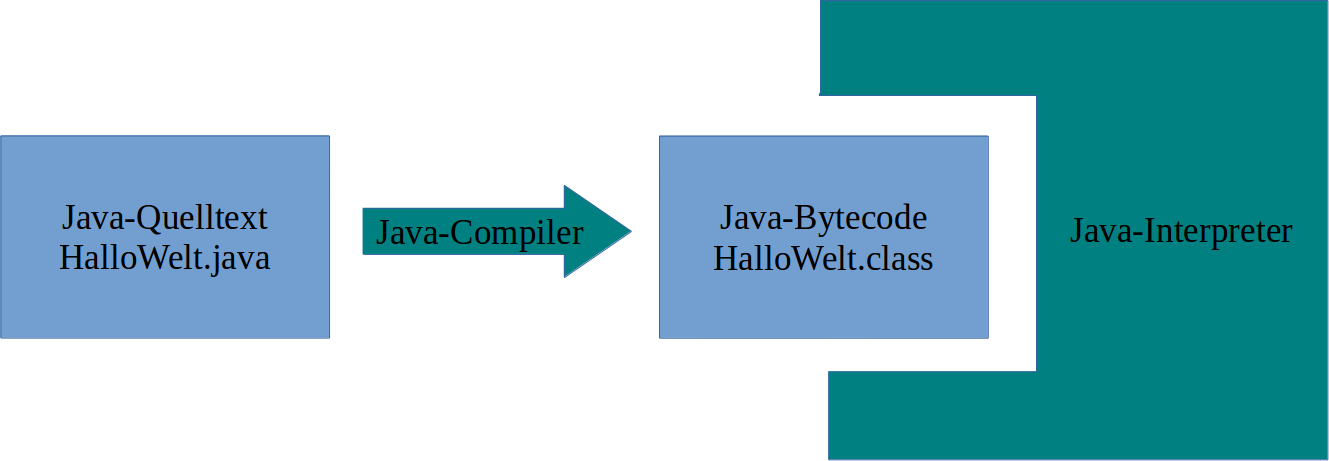
\includegraphics[width=0.8\textwidth]{grundl-java/Java-Kompiler}\\[2em]


\includegraphics[width=0.8\textwidth]{grundl-java/C++-Kompiler}

\begin{itemize}
 \item Java-Bytecode ist plattformunabhängig und kann vom Java-Interpreter auf jedem System ausgeführt werden.
 \item C++ Programme können direket vom Betriebssystem ausgeführt werden, wenn sie für dieses kompiliert wurden.
\end{itemize}

\end{frame}
